\newpage
\subsubsection{Flight Report: Secchi Disk}
\begin{minipage}{1\textwidth}
	\begin{flushright}
		Date: 13-06-2022, 12:00\\
		Weather: Sunny\\
		Location: Ton Duc Thang University\\
		Coordinates: 10.731373, 106.695396\\
		Flight Mode: \gls{GPS}\\
		Flight Duration: 15 minutes\\\vspace{5mm}
	\end{flushright}
\end{minipage}

The goal of this flight was to test if a secchi disk could be used in combination with drones to determine transparency of a water body. A secchi disk measurement is best performed from 10:00-14:00 on a sunny day.

The secchi disk with rope was attached to the drone as follows:

\begin{figure}[h]
\centering
\includegraphics[scale=0.07]{080_testing/flights/51_setup.jpg}
\caption{Secchi disk attached to the drone [own picture]}
\end{figure}


\paragraph{Calculation}
The drone was positioned in a way that the secchi disk just touched the water:

\begin{figure}[h]
\centering
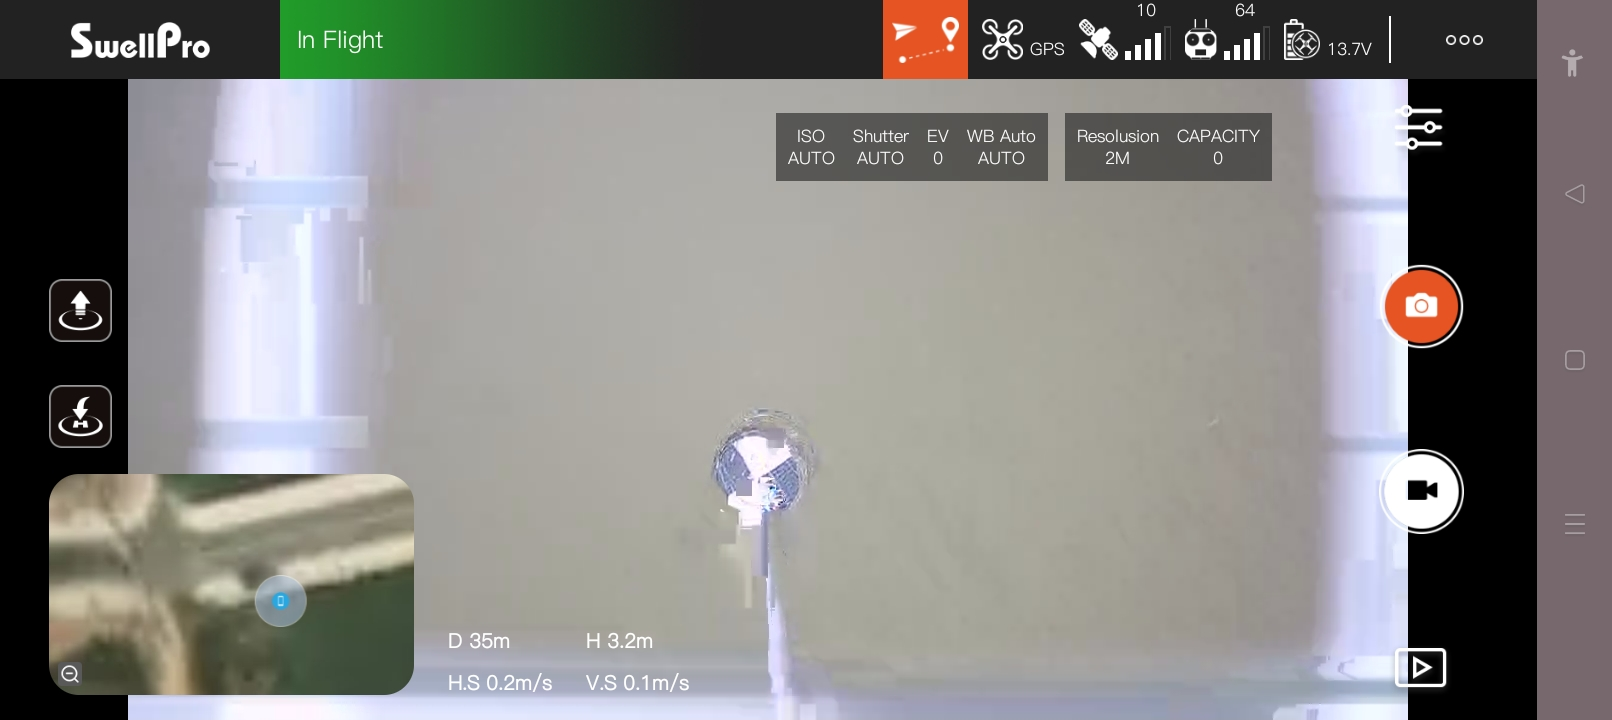
\includegraphics[scale=0.3]{080_testing/flights/52_screen1.jpg}
\caption{elevation 3.2 meter [own picture]}
\end{figure}

As seen in the screenshot above, the elevation of the drone was 3.2 meter. Lowering the drone, the secchi disk sunk in the water:

\begin{figure}[h]
\centering
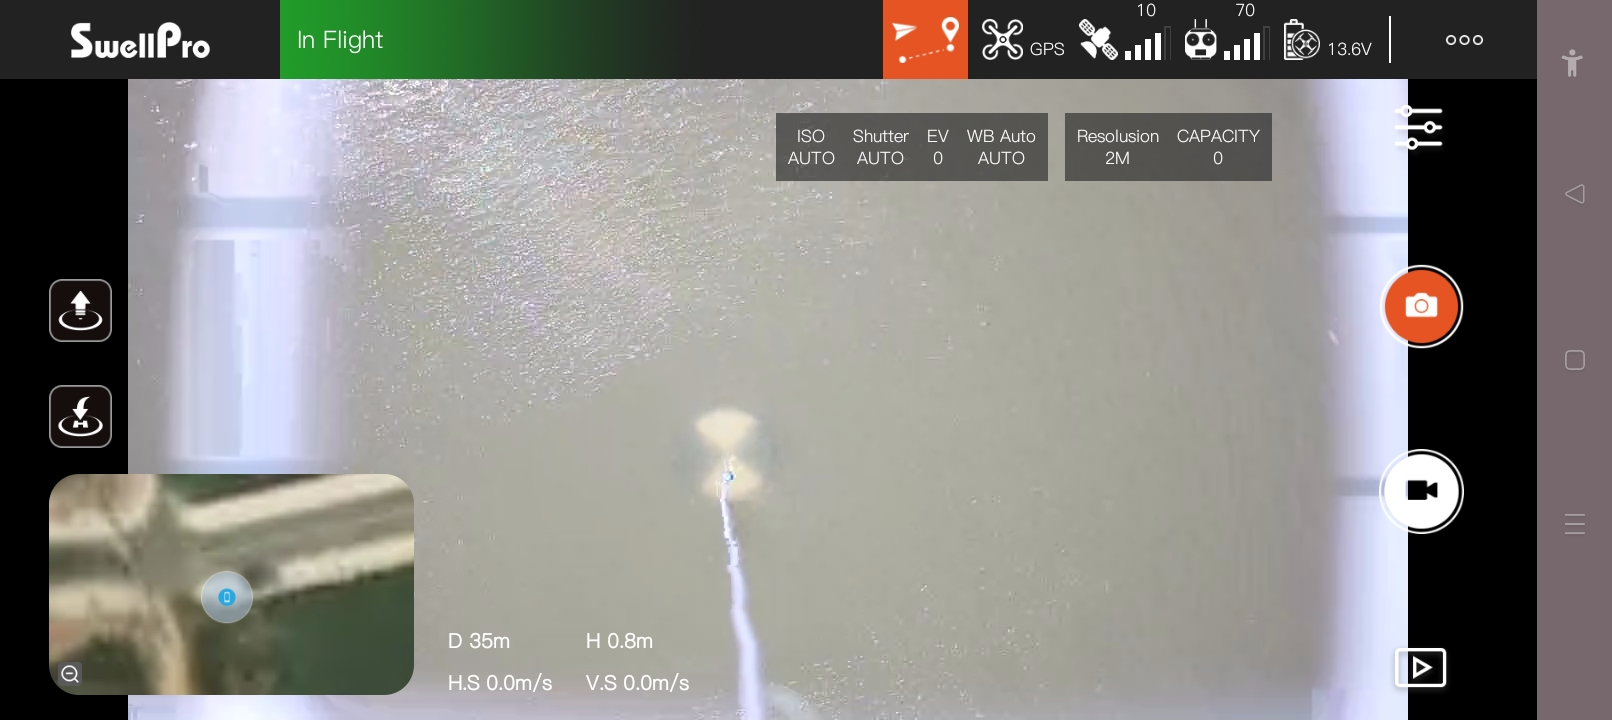
\includegraphics[scale=0.3]{080_testing/flights/53_screen2.jpg}
\caption{elevation 0.8 meter [own picture]}
\end{figure}

In this screenshot above one can see an elevation of 0.8 meter. One can see from the photo that the secchi disk is not that visible. Lowering the drone until the secchi disk disappears from sight:

\begin{figure}[h]
\centering
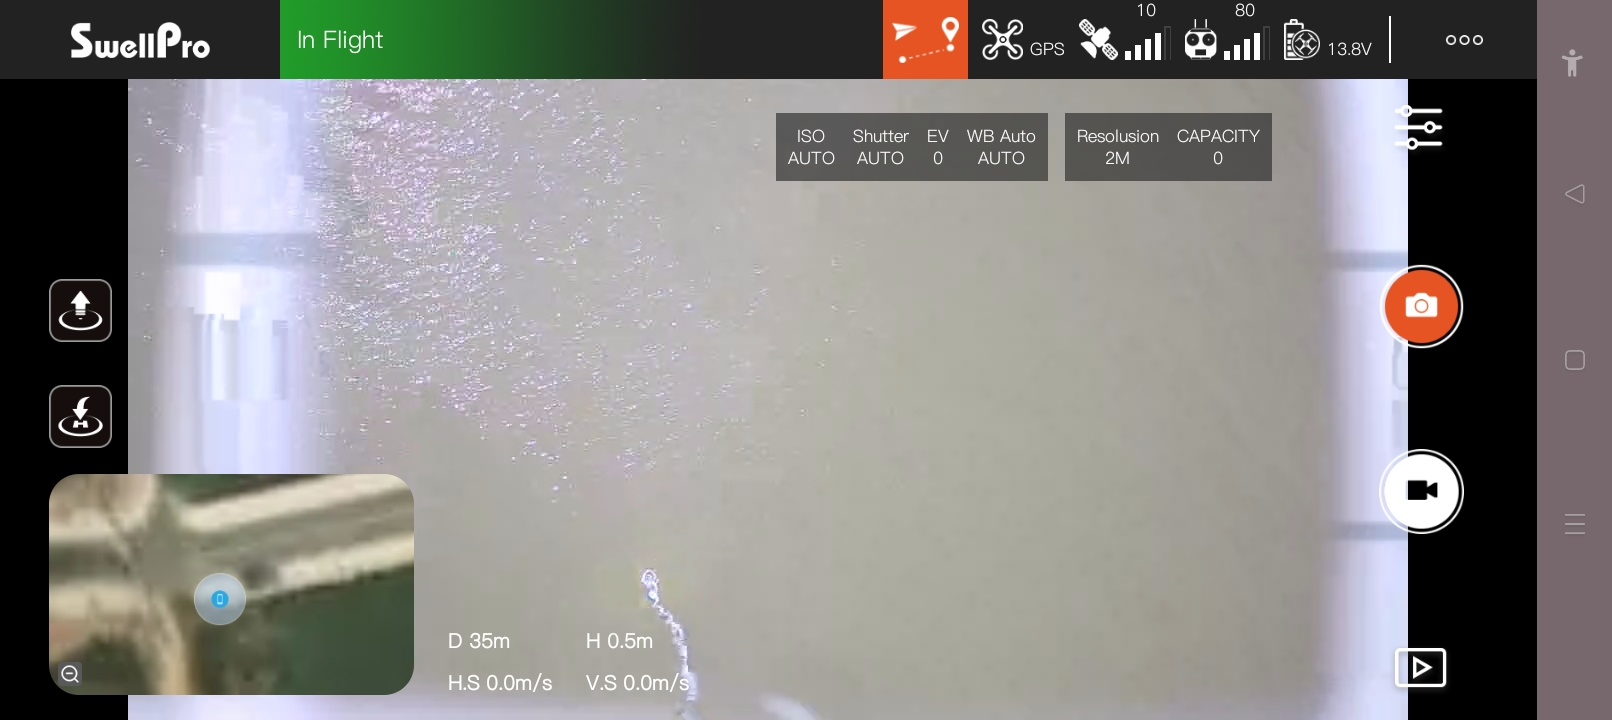
\includegraphics[scale=1.2]{080_testing/flights/54_screen3.jpg}
\caption{elevation 0.5 meter [own picture]}
\end{figure}

As seen, the disappearance elevation is at 0.5 meter. When a secchi disk is lowered vertically into the water the depth below the surface at which it just disappears from sight is called the secchi depth. The secchi depth can be defined as follows:
\[ Secchi depth = begin elevation - dissappear elevation \]
Giving a secchi depth of $3.2-0.5=2.7 meter$\\

Measuring the secchi depth manually gave a secchi depth of about 2.5 meter.

\paragraph{Battery life}
The drone had a heavy payload, so the battery life was significantly reduced from 30 minutes to 15 minutes. A lighter payload could be used in the future to improve battery life as long as it defeats buoyancy

\paragraph{Stability}
The drone managed to carry the secchi disk in mid air without any issues. Care had to be taken however in order for the rope to not swing too much in the air.

\paragraph{Conclusion}
Automated flights using the secchi disk may become a problem due to battery life and stability. Comparing manual and drone secchi disk, it is safe to conclude that the differences are within the margin of error normally present in secchi disk measurements.